% !TeX root = ../main.tex

\chapter{需求分析}
本章基于系统级仿真建模的基本需求,在此基础上,按照后续设计空间探索的
需求以及保证仿真平台性能的非功能需求,对仿真平台以及设计空间探索流程
的需求分析进行了详细的阐述。需求分析是非常关键以及重要的一步,为后续
应用的具体实现有着指导作用。

\section{系统需求分析简介}
基于Simpy的仿真平台是一个轻量级的系统级仿真平台,需要完成对原有业务行
为的仿真,可以适配现有的复杂的基于SystemC的SAE仿真平台的输入(例如任
务用例、硬件配置文件等等)。这个仿真平台只是针对于部门内部员工进行使
用,我们需要输出在用例仿真的时候一些硬件平台的具体信息(如核一段时间
的利用率、内存碎片等等)和任务执行的具体细节。仿真平台也需要支撑后续
的设计空间探索流程的实现。为了设计空间探索流程能够更简易使用,我们需
要将整个流程做成可配置的。

在平台设计的时候,设计人员对各个硬件模块有相应的功能需求。在我设计的模块中,
主要包含GeneralFifo模块、Processor模块以及Memory模块。这几个模块的功能需求
如表3.1所示:
\begin{table}[]
    \centering\normalsize
    \caption{硬件模块功能需求列表}
    \begin{tabular}{|c|c|}
    \hline
    模块            & 需求说明                           \\ \hline
    GeneralFifo模块 & 能够完成消息队列基础功能及事件触发              \\ \hline
    Processor模块   & Processor模块各种模型的功能正确、与其他模块成功交互 \\ \hline
    Memory模块      & 数据存取时序正确且数据不丢失、与其他模块成功交互       \\ \hline
    \end{tabular}
    \end{table}

在硬件模块设计过程中,设计人员需要完成对各个模块的功能需求的实现,保证模型在实例化
时能够成功搭建且保证功能正确,并且实现各个模块的执行流程细节在日志中可视。

在平台使用过程中,针对不同员工工作性质的不同,他们对仿真平台的需求也不同。
结合上述功能和针对不同用户进行分析,得出用户需求列表3.2。在这里我们将只使用仿真
平台运行用例的员工对应为普通用户1,需要配置硬件平台执行用例的员工对
应为高级用户,需要执行设计空间探索流程的员工对应为普通用户2。

\begin{table}[htb]
    \centering\normalsize
    \caption{用户需求列表}
    \begin{tabular}{|c|c|c|ll}
    \cline{1-3}
    ID    & 需求说明         & 需求来源       &  &  \\ \cline{1-3}
    UR1   & 执行用例文件       & 普通用户1、高级用户 &  &  \\ \cline{1-3}
    UR1.1 & 执行过程的异常报错    & 普通用户1、高级用户 &  &  \\ \cline{1-3}
    UR1.2 & 修改硬件平台配置     & 高级用户       &  &  \\ \cline{1-3}
    UR1.3 & 硬件模型扩展开发     & 高级用户       &  &  \\ \cline{1-3}
    UR2   & 读取用例执行结果     & 普通用户1、高级用户 &  &  \\ \cline{1-3}
    UR3   & 执行设计空间探索流程   & 普通用户2      &  &  \\ \cline{1-3}
    UR3.1 & 配置设计空间       & 普通用户2      &  &  \\ \cline{1-3}
    UR3.2 & 配置进化算法参数     & 普通用户2      &  &  \\ \cline{1-3}
    UR4   & 设计空间探索结果对比结果 & 普通用户2      &  &  \\ \cline{1-3}
    \end{tabular}
    \end{table}

\section{功能性需求}
功能需求主要用来列举用户对产品所预期的功能和服务。本产品主要的功能是进行
系统级业务行为仿真以及对整个系统架构的一些方面进行自动化的设计空间探索,
因此需要通过需求分析对不同用户所需要的功能进行分析和阐述。

首先,我们根据表3.1依次从GeneralFifo模块、Processor模块和Memory模块三个方面
对这三个模块的功能需求进行详细的阐述:

\subsection{GeneralFifo模块功能需求}
GeneralFifo模块在仿真平台中的功能是一个可以即时触发event的先入先出消息队列。它
需要满足接口可见且队列存取event可被其他模块触发的功能。该模块的用例图如下图
3.1所示:

\begin{figure}[h]
    \centering
    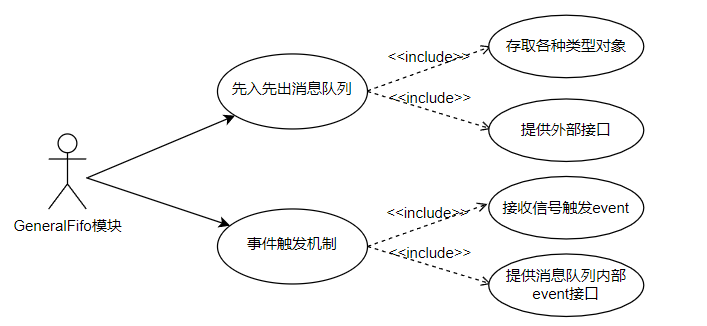
\includegraphics[width=0.75\textwidth]{GeneralFifo用例图.png}
    \caption{GeneralFifo模块用例图}
    \label{fig:badge}
\end{figure}

图3.1列举了GeneralFifo模块的功能需求。GeneralFifo作为一个先入先出队列需要满足
先入先出队列的所有功能,能够存储各种类型的对象,提供队列内部的一些基础接口如:
队列深度、存对象方法以及取对象方法等等。其次,GeneralFifo为了满足仿真平台能够
实现各个模块之间即时的消息传递,GeneralFifo需要实现当队列接收到消息时,便触发
相应的事件的功能,并且GeneralFifo模块需要提供模块内部的事件相关接口,以便其他模块
可以接受到队列内部的事件触发。

\subsection{Processor模块功能需求}
Process模块包括DSP、HAC以及DMA三种不同的硬件模型,Processor模块需要实现各个硬件
模型各自的功能需求以及硬件模块与其他模块之间的交互功能。Processor模块的用例图如
下图3.2所示:

\begin{figure}[h]
    \centering
    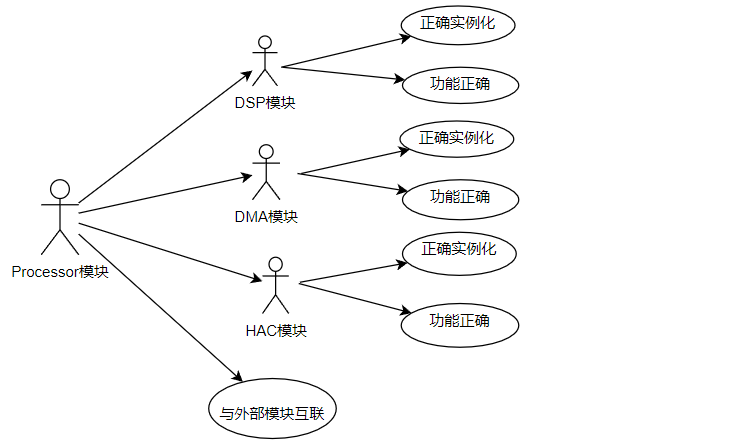
\includegraphics[width=0.75\textwidth]{Processor模块用例图.png}
    \caption{Processor模块用例图}
    \label{fig:badge}
\end{figure}

图3.2列举了Processor模块的整体需求,包括DSP、HAC和DMA三种硬件模型的功能需求以及
所有硬件模型与其他模块的交互功能需求,包含与Memory模块和调度器模块的交互。下面就
这几个方面分别来详细介绍Processor模块的功能需求。

DSP模块需要实现在仿真平台构建时,根据硬件平台配置文件中的信息正确实例化,保证
具体DSP实例能够通过总线连接到整个仿真平台中且DSP实例的配置信息正确。同时DSP模块
在实例化后需要实现自己的硬件功能:接收并处理来自DMA实例或者调度器模块
的任务实例,并根据任务实例中提取出的信息正确执行任务,并发送消息到下一级硬件实例
中。

HAC模块与其他Peocessor模块的一样需要在仿真平台构建时能够正确实例化。同时HAC模块
在实例化后需要实现自己的硬件功能,HAC模块作为一个用于处理某一种特定的任务的硬件
模块,其需要接收并处理来自调度器的任务实例。接收需要根据任务信息从特定地址的内存
块取出数据,然后以一定的时延处理任务,并在任务处理结束后将数据存储到特定地址的内
存中。在这个过程中需要保证任务处理时延正确、搬入搬出的数据正确。

DMA模块同样需要在仿真平台实例化的时候能够正确实例化。与此同时,DMA模块需要完成
其模块的功能,即与Memory模块进行交互,进行数据的搬入搬出,保证在数据的搬入搬出的
过程中数据的正确。并且DMA模块能够和其他模块进行消息交互,与DSP模块之间形成任务的
执行流水线。

Processor模块需要能与其他模块进行消息以及数据的交互,需要保证消息传递的及时性
以及正确性,保证数据传输时源地址和目的地址的正确以及数据本身的正确。

\subsection{Memory模块功能需求}
Memory模块需要实现能够成功实例化且模块功能正确,以及需要保证能够和其他模块进行
消息交互以及数据传输的功能。Memory模块的用例图如下图3.3所示:

\begin{figure}[h]
    \centering
    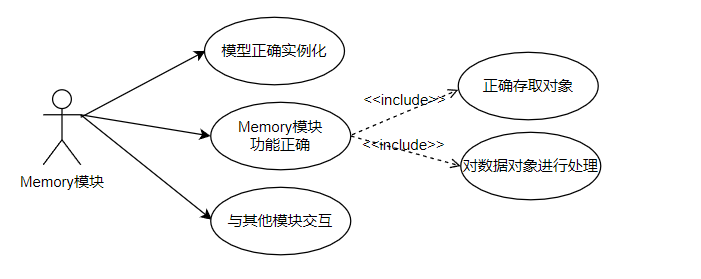
\includegraphics[width=0.75\textwidth]{Memory模块用例图.png}
    \caption{Memory模块用例图}
    \label{fig:badge}
\end{figure}

如图3.3所示,Memory模块需要实现模型能够正确实例化、Memory模块基础功能以及外部模块
之间消息交互的功能。这几部分需求的具体内容如下:

1、Memory模块能够在硬件平台搭建时根据硬件平台配置文件的信息去实例化,并通过
模块上实例化的Port与总线连接,从而与整个硬件平台连接在一起。

2、Memory模块需要保证其在实例化后,Memory实例的功能正确:Memory模块能够接收来自其他模块的
存取对象的请求,并根据请求的类型以及具体任务信息执行任务,在执行数据的存取时保证数据以及存取
地址的正确性。

3、Memory模块在执行数据存取的时候需要通过总线与其他内存模块进行数据的交互、通过GeneralFifo
消息队列与调度器模块中的内存管理模块、DMA实例以及HAC实例进行消息的交互,通知数据存取任务的
开始以及结束。

在介绍完仿真平台中硬件平台的功能需求之后,我们从仿真平台的使用用户的角度来介绍仿真平台的功
能性需求。如表3.2所示,仿真平台使用所涉及到的需求用户分为普通用户1、高级用户和普通用户2三类。
下面将对这三种用户的需求进行详细的分析。

\subsection{普通用户1需求}
普通用户1即是简单使用仿真平台进行业务仿真的用户。普通用户1的用例图如下
图3.4所示:

\begin{figure}[h]
    \centering
    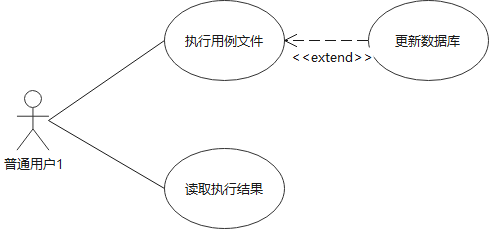
\includegraphics[width=0.75\textwidth]{普通用户1用例图.png}
    \caption{普通用户1用例图}
    \label{fig:badge}
\end{figure}

图3.4列举了普通用户1对仿真平台的执行用例文件功能、读取执行结果功能以及
仿真结果及仿真执行信息数据存储的需求,接下来对每个功能的具体需求进行阐述。
普通用户1的执行用例文件用例图如图3.5所示:

\begin{figure}[h]
    \centering
    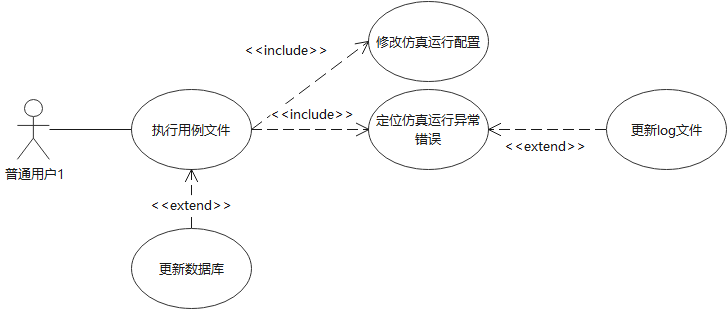
\includegraphics[width=1\textwidth]{普通用户1执行用例文件用例图.png}
    \caption{普通用户1执行用例文件用例图}
    \label{fig:badge}
\end{figure}

如图3.5执行用例文件用例图所示。执行用例文件功能分为修改仿真运行配置、
定位仿真运行异常错误和查看用例执行结果信息几个子功能。执行用例文件功
能及其子功能的需求具体内容如下:

1、	仿真结果时序正确。仿真时序正确要求每个任务的执行时间以及整体任务的
执行调度顺序与输入的任务用例文件中任务信息以及任务间的依赖关系一致。仿真
执行的输入是用例Excel文件,用例文件是将真实的任务在单板上的执行流程、执行
信息以及执行结果体现在文件中,通过解析文件信息,将任务真实的具体信息及依赖
关系作为仿真输入,通过任务调度平台的正确调度使得整个仿真最终得以正确执行。

2、	仿真运行可配置。因为我们需要的执行用例主要用于基带芯片上,所以用例可
能存在多小区多信道的用例同时执行或者不同的用例同时混合执行,所以我们需要
在仿真运行前配置用例执行次数、仿真执行的用例文件名称、硬件配置文件名称以
及log文件和数据库文件的位置,这样就能适配不同情况下的仿真。用户可以仅仅
、修改执行脚本中的数据即可对整个仿真执行过程进行修改,从而得出用户所需的
不同的仿真结果。

3、	定位仿真执行异常错误。任务用例在仿真过程中可能会遇到各种情况的错
误,有些是用例文件的任务信息错误,有些是任务执行时的错误。我们需要能
够迅速定位到错误位置,我们通过任务执行过程中细致的log记录,可以迅速
定位到任务执行哪一级出现错误以及可以查询到各个模块之间数据传输在总线
上哪一级出现问题,可以迅速地定位到问题的产生地方以及解决问题。

以上详细的介绍了普通用户1对仿真平台执行仿真用例的具体需求,包括在仿真过程
中通过数据库将详细的任务执行信息记录下来。

用户执行用例仿真的最终需求还是为了得到用例仿真结果信息。我们在仿真过
程中通过数据库记录硬件平台的具体信息(如核一段时间的利用率、内存碎片
等等)和任务执行的具体细节(任务的提交时间、开始时间、结束时间等等)。
用户可以通过访问数据库文件来查看用例执行结果信息,从而得出自己所需要的
的信息。数据库文件需要记录多次的仿真结果,不同的仿真结果以SimId为标志区
分,并记录仿真执行的平台、仿真的时钟频率、执行的用例文件等等该次仿真的具
体信息。这样我们可以将我们需要的执行的多次用例通过脚本依次执行,最后也可以
查看到每次仿真执行后的具体信息。

\subsection{高级用户需求}
高级用户即是那些深度使用和开发该仿真平台的用户,除了普通用户1的需求,
他们还需要对仿真平台的配置修改需求。高级用户的用例图如下图3.6所示:

\begin{figure}[h]
    \centering
    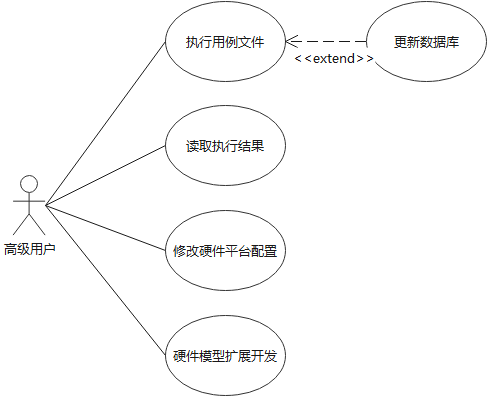
\includegraphics[width=0.7\textwidth]{高级用户用例图.png}
    \caption{高级用户用例图}
    \label{fig:badge}
\end{figure}

图3.6列举了高级用户仿真运行、读取仿真运行结果信息、修改硬件平台配置
和硬件模型扩展开发的需求。接下来我们对高级用户比普通用户1多出的两种
功能需求进行详细的阐述。

因为在芯片设计过程中,高级用户需要尝试手动修改仿真平台中硬件平台中不
同的硬件配置去运行仿真,因此我们的硬件配置需要高级用户能够很方便能够
去修改。仿真平台中硬件平台的构建是通过解析输入的硬件配置文件来进行的,
仿真平台输入的硬件配置文件类型包括Excel表及XML文件,用户可以通过
修改硬件配置文件中的硬件配置信息来达到他们对硬件配置进行修改的需求。

高级用户包括仿真平台的开发人员,芯片上的硬件不是统一不变,不同的硬件
行为不同,因此当出现不同的硬件时,我们需要对新的硬件进行建模。但现有
的芯片中的硬件类型大致就几种,我们基于硬件类型对各种硬件进行区分,为了这
种建模操作更加方便,我们统一构建了各种类型硬件的基类,建模时用户只需基于
这几种基类进行扩展开发即可。这样高级用户就可以很方便的仿真平台进行二次开发。

\subsection{普通用户2需求}
普通用户2即是那些使用设计空间探索流程的开发人员,他们只关注设计空间探
索流程的输入输出以及一些参数设置。普通用户2的用例图如下图3.7所示:

\begin{figure}[h]
    \centering
    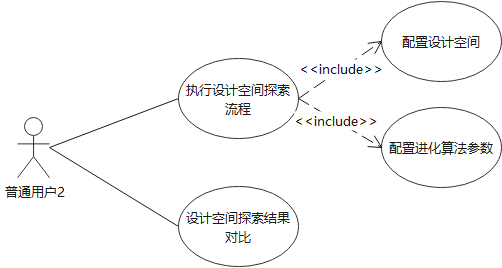
\includegraphics[width=0.8\textwidth]{普通用户2用例图.png}
    \caption{普通用户2用例图}
    \label{fig:badge}
\end{figure}

由图3.7可见,普通用户2关注设计空间探索流程的输入输出以及流程中一些
参数设置,对设计空间探索流程中具体执行过程并不关心。设计空间探索流
程的输入是目标值及其组成的设计空间和仿真模型。在流程中可以调整一些
进化算法的参数,如进化算法代数以及交叉变异的概率等等。我们通过在设
计空间探索流程执行脚本中设置相应的参数,就可以方便的调整设计空间探
索流程中遗传算法模块相应的参数,去得到对应的结果。最后能输出一
个种群的帕累托最优解集。

普通用户2可以通过设置的结果分析脚本使最后输出的脚本与原设计参数下执行结果进行对比,更加方
便可视化的得出用户所需要的结论。以便用户得出所需的设计参数或者进行下一轮的设计空间探索流程,
接下来对系统的非功能需求进行阐述。

\section{非功能需求}
仿真平台及设计空间流程整个系统在满足功能需求的基础上,还要根据系统的
实际情况,满足非功能需求。对于整个系统而言,非功能需求主要体现在可扩
展性、可维护性和性能需求上。这些非功能需求的作用对项目来说也是至关重
要的,只有同时满足功能性需求和非功能性需求,该应用才能在项目中顺利地
发挥其作用。

\subsection{可扩展性需求}
系统主体的仿真平台整体逻辑比较复杂,涉及5大模块,在各个模块内部有很多
部分功能类似,代码复杂,有很多模块需要复用。同时由于硬件设计的变化,
我们需要对硬件模块在后续开发中要不断进行扩展,整个项目的可扩展性要求
高,所以为了实现可扩展性需求,我们将各大模块代码模块化处理,在外部设
计接口,统一通过接口进行交互。模块内部功能相似的模块统一设计基类,通
过继承基类进行扩展开发。减少代码之间的循环依赖和降低代码之间的耦合,
从而提高系统的开发效率以及后续的扩展功能,使得系统满足可扩展性需求。

\subsection{可维护性需求}
在仿真建模以及仿真平台的搭建过程中,系统功能的实现并不能一劳永逸,在
新的硬件模块的增加后,仿真平台的功能以及性能是否满足要求,需要后续的
不断对其进行维护,才能保证仿真平台的稳定性和可用性。为了实现仿真平台
的可维护性,我们通过将仿真平台功能组件化,以保证后续模型的添加在功能
实现方面可以实现复用,更好的兼容现在的平台。降低了模型的开发难度以及
方便了后续开发人员对功能和组件的维护,提高了开发效率。

同时,因为仿真平台的输入也一直在变,我们设置了一个迭代平台,可以每天
在服务器上进行不同用例的自动化仿真,并给出仿真结果,降低了开发人员的
人工成本。

\subsection{性能需求}
仿真平台主要是为了进行业务行为仿真,设计空间探索的目的是为了得到在各个方面
结果都表现优秀的设计方案解集。所以评价仿真平台性能的指标包括仿真结果的时序
准确以及仿真执行的速度,评价设计空间探索流程的性能是观察其输出结果是
否在各个方面都体现了优秀的性能以及设计空间探索流程的效率。在这里我们
也将这些作为性能需求的评价指标。

首先,在仿真平台方面,我们将输入的用例文件解析为以任务和数据为节点的
有向无环图,这保证了任务执行的顺序,任务执行时间的准确则体现了硬件模
型行为的准确。为了仿真能够更快的执行,我们简化了硬件模型的行为,以软
件行为替代硬件行为,在内存模型上我们简化了数据的格式,将真实的数据存
取过程只是体现在仿真时延的增加,而不是真实的进行存取。且采用了Simpy
仿真框架,从而实现仿真速度的提升。

其次,在设计空间探索方面,我们采用进化算法,并通过进化算法的选择和具体
的算法设置保证结果是全局最优而不会陷入局部最优。我们同时也需要保证设计
空间探索流程的速度,保证整个设计空间探索流程能在很短时间闭环,以方便设
计人员能在设计空间探索流程结束后很快的对设计探索的结果进行分析,得出所
需要的设计架构。由于我们采用进化算法,我们在每一代中,对于相应的参数,
我们都要通过仿真得到对应的仿真结果并且提取出我们需要的结果。因此我们通
过在设计空间探索过程中将仿真模型通过机器学习简化为仿真预测模型,这样能
大大减少每一次的对对应设计参数得出结果的时间,从而达到极大的提高设计空
间探索流程的效率的需求。性能需求表如下表3.3所示:

\begin{table}[htb]
    \centering\normalsize
    \caption{性能需求表}
    \begin{tabular}{|c|c|c|ll}
    \hline
    模块       & 需求项           & 需求值               \\ \hline
    仿真平台构建模块 & 仿真硬件平台搭建成功的时间 & \textless{}=5s    \\ \hline
    仿真执行模块   & 单次单小区仿真执行的时间  & \textless{}=15s   \\ \hline
    仿真执行模块   & 仿真结果时序与用例一致   & true              \\ \hline
    设计空间探索模块 & 单次一代遗传算法执行时间  & \textless{}=500ms \\ \hline
    设计空间探索模块 & 设计空间探索结果全局最优  & true              \\ \hline
    \end{tabular}
    \end{table}

\section{本章小结}
本章从实际场景出发,根据业务仿真的真实场景和设计空间探索流程的真实场景
,详细分析了整个系统的功能需求和非功能需求,在对产品的需求进行了简介之
后,给出了用户需求列表。在功能需求中,根据不同用户对系统的需求,对功能
需求进行了详细的阐述,描述了用例文件执行、查看仿真结果信息、执行设计空
间探索流程和得到设计空间探索结果对比等功能需求。接着根据系统的实际情况,
从可扩展性、可维护性和性能需求几个方面来详细阐述系统的非功能需求。
这一章对仿真平台及设计空间探索流程的需求进行了比较明确地阐述,为后续的
系统概要设计打下了基础。